%In this section we will reinterpret Adams spectral sequence vanishing lines in terms of synthetic spectra and prove several genericity statements. 
%
This section begins our study of vanishing lines in Adams spectral sequences, which is subject of Sections \ref{sec:AppendixVL}-\ref{sec:mod8} and \Cref{sec:Appendix}. In this section, our main concern will be the genericity properties of various notions of vanishing lines in synthetic spectra. A key feature of our methods is that they make clear how the intercepts of such vanishing lines change in cofiber sequences. Our results are used in \Cref{sec:ANvl} to obtain an explicit vanishing line in the Adams-Novikov spectral sequence for the $p$-local sphere, for each $p \ge 3$. In \Cref{sec:Appendix} the results of Sections \ref{sec:AppendixVL} and \ref{sec:ANvl} are used to deduce \Cref{thm:Burklund}(2).

Our genericity results recover versions of the genericity results of Hopkins, Palmieri and Smith \cite{HPS} for finite-page vanishing lines in $E$-Adams spectral sequences.  One side effect of our use of synthetic spectra is that we only prove results for $E$ of Adams type.

%revisit work on vanishing lines in Adams spectral sequences from the perspective of synthetic spectra. In particular, we will prove a version of the main result of \cite{HPS} on the genericity of vanishing lines in Adams spectral sequences. The synthetic viewpoint makes the proof particularly perspicuous and allows us to make certain constants left inexplicit in \cite{HPS} precise. \todo{Mention that we assume Adams type.}

%%---------- Definitions------------

%\begin{dfn}
%  \todo{need to decide whether to use this or just img(nu)}
%  Let $Syn_E^{\text{eff}}$ denote the full subcategory of synthetic spectra generated under colimits and extensions by $\{\nu Y\}$ for $Y \in \Sp_{\geq 0}^{fp}$. \todo{is this the right name for this?}
%\end{dfn}

%We begin by recalling with what it means for a property of (synthetic) spectra to be generic.

\begin{dfn}
  A \emph{thick subcategory} $\mathcal{C}$ of $\Sp$ (resp. $\Syn_E$) is a full subcategory which satisfies the following properties:
  \begin{itemize}
  \item it is closed under suspensions $\Sigma^n$ (resp. $\Sigma^{p,q}$) for $n,p,q \in \Z$,
  \item it is closed under retracts,
  \item if $X \to Y \to Z$ is a cofiber sequence and any two of $X,Y,Z$ are in $\mathcal{C}$, then so is the third.
  \end{itemize}

  Following \cite[Definition 1.1]{HPS}, we say that a property of (synthetic) spectra is \emph{generic} if the full subcategory of (synthetic) spectra satisfying that property is thick.
\end{dfn}

We now define four notions of vanishing line.

\begin{dfn}
  Given a synthetic spectrum $X$, we will say that
  \begin{enumerate}
  \item $X$ has a vanishing line of slope $m$ and intercept $c$
    if $\pi_{k,k+s}(X) = 0$ whenever $s > mk+c$.
  \item $X$ has a strong vanishing line of slope $m$ and intercept $c$
    if $X \otimes \nu_E (Y)$ has a vanishing line of slope $m$ and intercept $c$ for every connective spectrum $Y \in \Sp_{\geq 0}$.
    %\footnote{The compatibility of $\nu_E$ with filtered colimits implies that it suffices to check this for \emph{finite} $Y \in \Sp_{\geq 0}$.}
  \item $X$ has a finite-page vanishing line of slope $m$, intercept $c$ and torsion level $r$ 
    if every class in $\pi_{k,k+s}(X)$ is $\tau^r$-torsion when $s > mk+c$.
  \item $X$ has a strong finite-page vanishing line of slope $m$, intercept $c$ and torsion level $r$
    if $X \otimes \nu_E (Y)$ has a finite-page vanishing line of slope $m$, intercept $c$ and torsion level $r$ for every $Y \in \Sp_{\geq 0}$.
    %\footnote{ditto}
  \end{enumerate}
\end{dfn}

\begin{rmk}
    The compatibility of $\nu_E$ with filtered colimits implies that the presence of a strong (finite-page) vanishing line need only be checked on \emph{finite} $Y \in \Sp_{\geq 0}$.

\end{rmk}

\begin{rmk}
  \label{rmk:strict-as-pc}
  A (strong) vanishing line of slope $m$ and intercept $c$ is equivalent to a (strong) finite-page vanishing line of slope $m$, intercept $c$ and torsion level $0$.
\end{rmk}

\begin{rmk}
    Given an $E$-nilpotent complete spectrum $X$, we will say that the $E$-based Adams spectral sequence for $X$ admits a (strong) (finite-page) vanishing line if $\nu_E (X)$ does. This is justified by the following proposition.
\end{rmk}

\begin{prop}\label{prop:vanishing-line-Adams}
    Given an $E$-nilpotent complete spectrum $Y$, $\nu_E (Y)$ admits a finite-page vanishing line of slope $m$, intercept $c$ and torsion level $r$ if and only if $\mathrm{E}^{s,k+s} _{r+2} = 0$ for $s > mk+c$.
\end{prop}

\begin{figure}
  \centering
    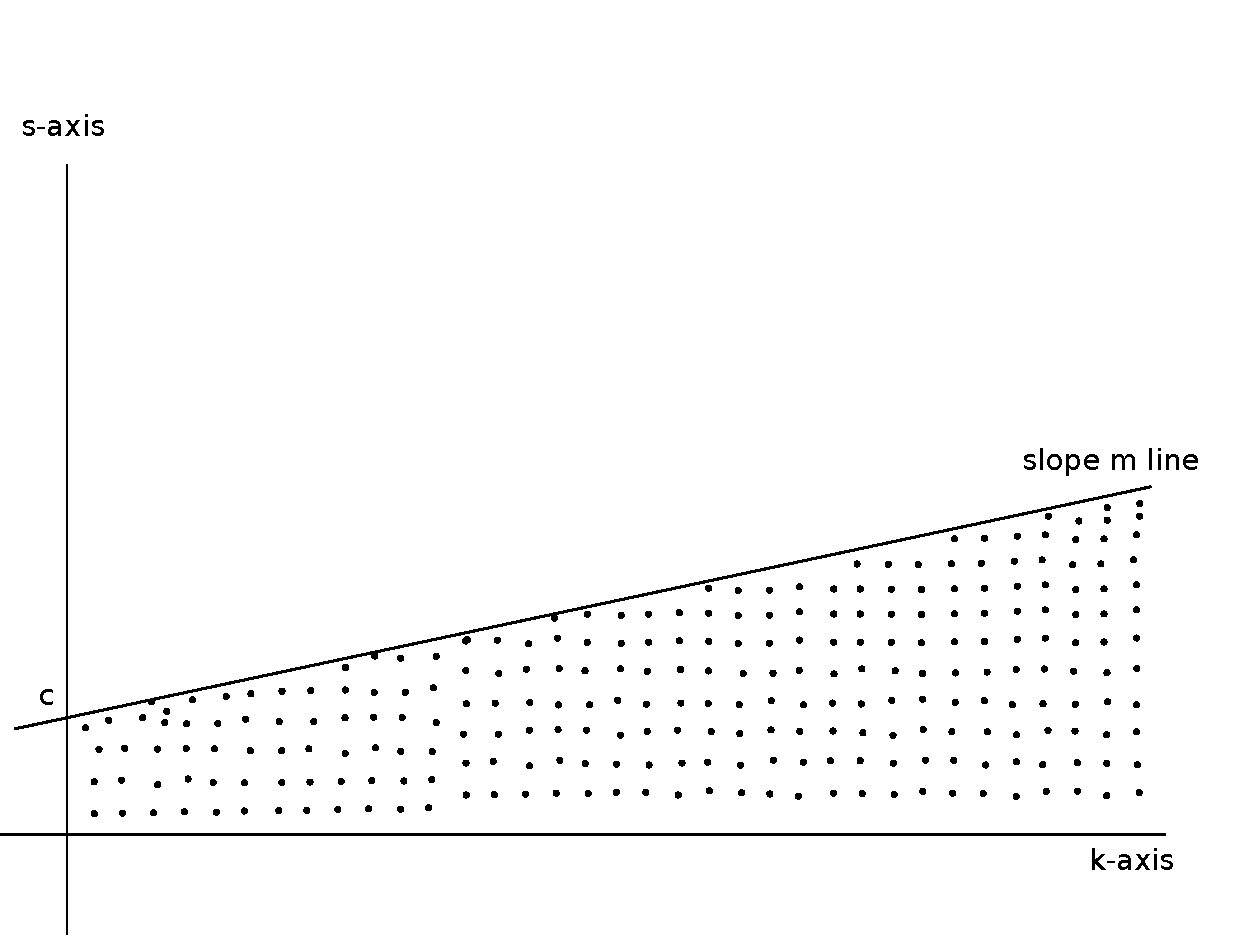
\includegraphics[scale=0.6]{vanishing-line-diagram.pdf}
    \caption{In this figure we display a picture of what the $\mathrm{E}_{r+2}$-page of the $E$-Adams spectral sequence of an $E$-nilpotent complete spectrum that admits a finite-page vanishing line of slope $m$, intercept $c$ and torsion level $r$ looks like. Namely, the region strictly above the vanishing line must consist of zero groups on the $\mathrm{E}_{r+2}$-page.}
    \label{fig:banded}
\end{figure}

We will need the following technical lemmas in the proof of \Cref{prop:vanishing-line-Adams}.

\begin{lem}\label{lemm:vanishing-line-converge}
    Given an $E$-nilpotent complete spectrum $Y$, the $E$-based Adams spectral sequence for $Y$ converges strongly if $\nu_E (Y)$ admits a finite-page vanishing line of positive slope.
\end{lem}

\begin{proof}
    By \Cref{cor:strong-conv}, it suffices to show that the $\tau$-Bockstein spectral sequence for $\nu_E (Y)$ converges strongly. By \Cref{thm:strong-conv}, to show strong convergence it will suffice to show that there are only finitely many differentials exiting each tridegree. But the finite-page vanishing line for $\nu_E Y$ implies that every $d_{s} ^{\tau-\mathrm{BSS}}$ with $s > r+1$ and target above the vanishing line must be zero. This implies that each group in the $\tau$-Bockstein spectral sequence may only be the source of only finitely many differentials, as required.
    %\cite[Theorem 7.1]{Boardman}.
\end{proof}

\begin{lem}\label{lemm:vanishing-converge}
    Let $Y$ denote an $E$-nilpotent complete spectrum and suppose that there exist numbers $m > 0$, $c$ and $r$ for which the $E$-Adams spectral sequence of $Y$ satisfies $\mathrm{E}^{s,k+s} _{r} = 0$ for $s > mk+c$. Then the $E$-Adams spectral sequence for $Y$ converges strongly.
\end{lem}

\begin{proof}
    It follows from the assumption that each group in the spectral sequence can only have finitely many differentials originating from it, so the result follows from \Cref{thm:strong-conv}.
    %\cite[Theorem 7.1]{Boardman}.
\end{proof}

\begin{proof}[Proof of \Cref{prop:vanishing-line-Adams}]
    Let $Y$ denote an $E$-nilpotent complete spectrum satisfying one of the conditions in the statement of the proposition. By either \Cref{lemm:vanishing-line-converge} or \Cref{lemm:vanishing-converge}, the $E$-Adams spectral sequence for $Y$ converges strongly. We are therefore free to invoke \Cref{thm:synthetic-Adams} in the following.

    Assume that $\nu_E (Y)$ admits a finite-page vanishing line of slope $m$, intercept $c$ and torsion level $r$, and suppose that there exists $0 \neq x \in \mathrm{E}^{s,k+s} _{r+2}$ with $s > mk +c$. If $x$ is the source of a differential, we may replace it by its target and therefore assume without loss of generality that $x$ is a permanent cycle. Let $y \in \mathrm{E}^{s,k+s} _2$ be a representative of $x$. Invoking \Cref{thm:synthetic-Adams}, we conclude that there exists $\wt{y} \in \pi_{s,k+s} (\nu_E Y)$ which is not $\tau^r$-torsion, a contradiction.

    Now suppose that $\mathrm{E}^{s,k+s} _{r+2} = 0$ when $s > mk+c$.  Applying \Cref{thm:synthetic-Adams}, we see that every element of the form $\wt{x}$ above the vanishing line is $\tau^r$-torsion. \Cref{thm:synthetic-Adams} also implies that the $\tau$-adic completion of the $\Z[\tau]$-submodule of the bigraded homotopy generated by such $\wt{x}$ is exactly $\pi_{*,*} (\nu_E Y)$. From the uniform bound on the $\tau$-torsion order, we learn that the completion was unnecessary. It follows that every class in $\pi_{k,k+s} (\nu_E Y)$ is $\tau^r$-torsion when $s > mk + c$, i.e. that $\nu_E Y$ admits a finite-page vanishing line of slope $m$, intercept $c$ and torsion level $r$.
\end{proof}

\begin{comment}
\begin{rmk}
    Note that a vanishing line is the same as a finite-page vanishing line of torsion level $0$, so the above proposition says that a vanishing line in $\nu_E (Y)$ corresponds to a vanishing line on the $\mathrm{E}_2$-page of the $E$-based Adams spectral sequence for $Y$.
\end{rmk}
\end{comment}

\begin{comment}
\begin{rmk}
    Given an $E$-complete spectrum $Y$, it follows from \Cref{lemm:Elocal-taucomplete}, \Cref{lemm:ctaugoodenough} and \Cref{lemm:ctauE2} that a vanishing line for $\nu_E (Y)$ corresponds to a vanishing line in the $\mathrm{E}_2$-page of the $E$-based Adams spectral sequence for $Y$. \Cref{thm:synthetic-Adams} implies that a finite-page vanishing line for $\nu(Y)$ of torsion level $r$ corresponds to a vanishing line on the $\mathrm{E}_{r+1}$-page of the $E$-based Adams spectral sequence.
\end{rmk}
\end{comment}

We now state the main result of this section.

\begin{thm}
  \label{thm:vl-are-generic}
  Given a slope $m>0$, the following four conditions on a synthetic spectrum $X$ are generic:
  \begin{enumerate}
  \item $X$ has a vanishing line of slope $m$.
  \item $X$ has a strong vanishing line of slope $m$.
  \item $X$ has a finite-page vanishing line of slope $m$.
  \item $X$ has a strong finite-page vanishing line of slope $m$.
  \end{enumerate}
\end{thm}

The proof of this theorem will be given over the course of two lemmas.

\begin{lem}
  \label{lemm:suspension-line}
  Suppose that a synthetic spectrum $X$ has a (strong) (finite-page) vanishing line of slope $m$, intercept $c$ and torsion level $r$. Then:
  \begin{enumerate}
  \item Any retract of $X$ has a (strong) (finite-page) vanishing line of slope $m$, intercept $c$ and torsion level $r$.
  \item $\Sigma^{k,k} X$ has a (strong) (finite-page) vanishing line of slope $m$, intercept $c-mk$ and torsion level $r$.
  \item $\Sigma^{0,s} X$ has a (strong) (finite-page) vanishing line of slope $m$, intercept $c+s$ and torsion level $r$.
  \end{enumerate}
\end{lem}

\begin{proof}
  The first claim follows from the fact that the bigraded homotopy groups of a retract of $X$ are a retract of the bigraded homotopy groups of $X$.
  The second and third claim follow from keeping track of the change in indexing of the bigraded homotopy groups under bigraded suspensions.
\end{proof}

\begin{lem}
  \label{lemm:cof-line}
  Given a cofiber sequence of synthetic spectra
  $$ A \xrightarrow{f} B \xrightarrow{g} C $$
  such that
  \begin{enumerate}
  \item $A$ has a (strong) (finite-page) vanishing line of slope $m$, intercept $c_1$ and torsion level $r_1$,
  \item $C$ has a (strong) (finite-page) vanishing line of slope $m$, intercept $c_2$ and torsion level $r_2$.
  \end{enumerate}
  Then, $B$ has a (strong) (finite-page) vanishing line of slope $m$, intercept $\max(c_1+r_2,c_2)$ and torsion level $r_1+r_2$.
\end{lem}

\begin{proof}
  Remark \ref{rmk:strict-as-pc} implies that it will suffice to prove the finite-page versions of this lemma. One can also easily see that the strong versions follow from the weak versions applied to all cofiber sequences of the form
  $$ A \otimes \nu_E (Y) \to B \otimes \nu_E (Y) \to C \otimes \nu_E (Y) $$
  where $Y \in \text{Sp}_{\geq 0}$.
  
%  The statement for plain vanishing lines follows immediately from the long exact sequences on bigraded homotopy groups.

  We finish the proof by proving the statement for finite-page vanishing lines. Suppose that $\alpha \in \pi_{k,k+s}(B)$ with $s > mk + \max(c_1+r_2,c_2)$. From the finite-page vanishing line for $C$ the class $g(\alpha)$ is $\tau^{r_2}$-torsion. Thus, there is a class $\alpha' \in \pi_{k,k+s-r_2}(A)$ such that $f(\alpha') = \tau^{r_2}\alpha$. By assumption, $s-r_2 > mk + c_1$, so the finite-page vanishing line for $A$ tells us that $\alpha'$ is $\tau^{r_1}$-torsion. In particular, $\tau^{r_1+r_2}\alpha = 0$, as desired.
\end{proof}

Combining \Cref{lemm:suspension-line} and \Cref{lemm:cof-line} gives the proof of \Cref{thm:vl-are-generic}.
We record the following corollary, which will find use in \Cref{sec:ANvl}.

\begin{cor} \label{cor:ctau-vl}
  The synthetic spectrum $C\tau^M$ has a strong finite-page vanishing line of slope $m$, intercept $c$ and torsion level $M$ for every slope $m$ and intercept $c$.
\end{cor}

\begin{proof}
  We proceed by induction on $M$.
  The base case follows from the fact that $C\tau$ is a ring \cite[Corollary 4.45]{Pstragowski} and therefore every $C\tau$-module has homotopy groups which are simple $\tau$-torsion. For $M > 1$, we apply \Cref{lemm:cof-line} to the cofiber sequences
  \[ \Sigma^{0,-1} C\tau^{M-1} \to C\tau^M \to C\tau. \qedhere \]
  %We just need to show that the bigraded homotopy groups of $C\tau^M$ are $\tau^M$-torsion. The case of $C\tau$ follows from the fact that $C\tau$ is a ring, which is . For $M > 1$, we use induct on $M$ by applying \Cref{lemm:cof-line} to the cofiber sequences \[\Sigma^{0,-1} C\tau^{M-1} \to C\tau^M \to C\tau. \qedhere\]
\end{proof}

Next we prove a version of \cite[Theorem 1.3]{HPS}.

\begin{thm}\label{thm:HPS}
  Given a slope $m > 0$, the following conditions on an $E$-local spectrum $X$ are generic:
  \begin{enumerate}
  \item $\nu_E (X)$ admits a finite-page vanishing line of slope $m$.
  \item $\nu_E (X)$ admits a strong finite-page vanishing line of slope $m$.
  \end{enumerate}
\end{thm}

\begin{rmk}
  Specializing to the case where $X$ is $E$-nilpotent complete, \Cref{prop:vanishing-line-Adams} and \Cref{thm:HPS}(1) together recovers a version of \cite[Theorem 1.3 (i)]{HPS}.

  Our assumptions on $E$ in \Cref{thm:HPS} differ from those given in \cite[Condition 1.2]{HPS}. We assume that $E$ is of Adams type, whereas \cite{HPS} assumes, among other things, that $E$ is connective.
\end{rmk}

%\begin{rmk}
%    Since $\nu_E$ is not in general symmetric monoidal, part (2) of \Cref{thm:HPS} above doesn't translate exactly to \cite[Theorem 1.3 (ii)]{HPS}.
%\end{rmk}

To deduce \Cref{thm:HPS} from \Cref{thm:vl-are-generic}, we need to bound the extent to which $\nu_E$ fails to preserve cofiber sequences.

\begin{comment}
\begin{lem}
  \label{lemm:strong=weak}
  If $E$ is one of $\F_p$ or $BP$,
  then a synthetic spectrum $X$ has a vanishing line of slope $m$ and intercept $c$ if and only if it has a strong vanishing line of slope $m$ and intercept $c$.
\end{lem}

\begin{proof}
  \todo{either prove this or mess with later statements.}
\end{proof}
\end{comment}

\begin{lem}\label{lemm:comparison-tau-tor}
  Let $X \to Y \to Z$ be a cofiber sequence of $E$-local spectra. Moreover, let $C$ denote the cofiber of $\nu_E (X) \to \nu_E (Y)$. Then the cofiber $D$ of the induced map $C \to \nu_E (Z)$ is a $C\tau$-module.
\end{lem}

\begin{proof}
	We may build a commutative diagram
	\begin{center}
	\begin{tikzcd}
		\nu_E (X) \arrow[r] \arrow[d, "\mathrm{id}_{\nu_E (X)}"] & \nu_E (Y) \arrow[r] \arrow[d, "\mathrm{id}_{\nu_E (X)}"] & C \arrow[r] \arrow[d] & \Sigma^{1,0} \nu_E (X) \arrow[r] \arrow[d, "\tau"] & \Sigma^{1,0} \nu_E (Y) \arrow[d, "\tau"] \\
		\nu_E (X) \arrow[r] & \nu_E (Y) \arrow[r] & \nu_E (Z) \arrow[r] & \nu_E (\Sigma X) \arrow[r] & \nu_E (\Sigma Y) 
	\end{tikzcd}
	\end{center}
    out of the comparison maps between colimits before applying $\nu_E $ and after. By \cite[Remark 4.61]{Pstragowski}, there is a natural isomorphism \[(\nu E)_{k,k+*} (\nu_E(W)) \cong E_{k} (W)[\tau]\] for any spectrum $W$. This is an isomorphism of bigraded groups if $E_k (W)$ is considered to have bidegree $(k,k)$ and $\tau$ is given bidegree $(0,1)$. Applying $\nu E_{*,*} (-)$, we obtain a diagram
	\begin{center}
    \begin{tikzcd}[column sep = small]
		E_{k} (X)[\tau] \arrow[r] \arrow[d,"\text{id}"] & E_{k} (Y)[\tau] \arrow[r] \arrow[d,"\text{id}"] & \nu E_{k,k+*} (C) \arrow[r] \arrow[d] & \Sigma^{0,-1} E_{k-1} (X) [\tau] \arrow[r] \arrow[d, "\cdot \tau"] & \Sigma^{0,-1} E_{k-1} (Y) [\tau] \arrow[d, "\cdot \tau"] \\
		E_{k} (X)[\tau] \arrow[r] & E_{k} (Y)[\tau] \arrow[r] & E_{k} (Z)[\tau] \arrow[r] & E_{k-1} (X) [\tau] \arrow[r] & E_{k-1} (Y) [\tau],
	\end{tikzcd}
	\end{center}
	where both the top and bottom rows are exact: the top is exact because it arose from applying $\nu E_{*,*}$ to a cofiber sequence, and the bottom is exact because it is obtained by adjoining $\tau$ to an exact sequence.
    Letting $f : E_{k} (X) \to E_k (Y)$ denote the map induced by $X \to Y$, we find that \[ 0 \to \nu E_{k,k+*} (C) \to E_k (Z) [\tau] \to \ker(f)_{k-1} \to 0 \] is exact. Recalling that we defined $D$ to be the cofiber of $C \to \nu_E (Z)$, we conclude that \[\nu E_{k,k+\ell} (D) = \begin{cases} \ker(f)_{k-1},& \text{if } \ell = 0\\ 0,& \text{otherwise.} \end{cases}\]
        This is sufficient to conclude that $D$ is a $C\tau$-module, from our assumptions that $X$, $Y$ and $Z$ are $E$-local. Indeed, this is a combination of citations to \cite{Pstragowski}. In the language of that paper $D$ is hypercomplete \cite[Propositions 5.4 and 5.6]{Pstragowski}. Therefore \cite[Theorem 4.18]{Pstragowski} implies that $D$ lies in the heart of the natural $t$-structure on $\Syn_E$, which is discussed in \cite[Section 4.2]{Pstragowski}.
        By \cite[Lemmas 4.42 and 4.43]{Pstragowski}, there is an adjunction $\epsilon_* : \mathrm{Syn}_E \leftrightarrows \mathrm{Stable}_{E_* E} : \epsilon^*$ with $\epsilon^*$ lax symmetric monoidal and which induces an equivalence on the hearts. It follows that $D \simeq \epsilon^* (\epsilon_* (D))$. Since $C\tau \simeq \epsilon^* (E_*)$ as $\mathbb{E}_{\infty}$-rings \cite[Corollary 4.45]{Pstragowski}, $D \simeq \epsilon^* (\epsilon_* (D))$ is a $C\tau$-module by lax symmetric monoidality of $\epsilon^*$.
%
        %It follows that $\tau : \Sigma^{0,-1} D \to D$ is null, since $\Sigma^{0,-1} D$ is $1$-connective and $D$ is $0$-truncated. We conclude that $D$ is a $C\tau$-module.
\end{proof}

\begin{cor}\label{cor:HPS}
	Let $A \to B \to C$ be a cofiber sequence of $E$-local spectra and suppose that
	\begin{enumerate}
		\item $\nu_E (A)$ has a (strong) finite-page vanishing line of slope $m$, intercept $c_1$ and torsion level $r_1$,
		\item $\nu_E (C)$ has a (strong) finite-page vanishing line of slope $m$, intercept $c_2$ and torsion level $r_2$.
	\end{enumerate}
	Then $\nu_E (B)$ has a (strong) finite-page vanishing line of slope $m$, intercept $\max(c_1+r_2, c_2)+1$ and torsion level $r_1 + r_2 + 1$.
\end{cor}

\begin{proof}
	By \Cref{lemm:cof-line}, the cofiber $X$ of $\nu_E (\Sigma C) \to \nu_E (A)$ has a (strong) finite-page vanishing line of slope $m$, intercept $\max(c_1+r_2, c_2)$ and torsion level $r_1 + r_2$. By \Cref{lemm:comparison-tau-tor}, the cofiber $Y$ of $X \to \nu_E (B)$ is a $C\tau$-module. It follows that $Y$ has a strong finite-page vanishing line of slope $m$, arbitrary negative intercept and torsion level $1$.

	Applying \Cref{lemm:cof-line} to $X \to \nu_E (B) \to Y$, we obtain the desired result.
\end{proof}

\begin{proof}[Proof of \Cref{thm:HPS}]
	This follows from \Cref{cor:HPS}, \Cref{lemm:suspension-line} and the fact that $\nu_E$ sends retracts to retracts and suspensions to bigraded suspensions.
\end{proof}

Finally, we record a lemma which is useful in establishing (strong) vanishing lines. We say that a synthetic spectrum is $\tau$-complete if the natural map $X \to \varprojlim X \otimes C\tau^{n}$ is an equivalence.

\begin{lem} \label{lemm:vl-ctau}
	A $\tau$-complete synthetic spectrum $X$ has a vanishing line (resp. strong vanishing line) of slope $m \geq 0$ and intercept $c$ if and only if $X \otimes C\tau$ does.
\end{lem}

\begin{proof}
  The ``only if'' direction is easy and follows from considering the exact sequence
  $$ \pi_{a,b}(X) \to \pi_{a,b}(X \otimes C\tau) \to \pi_{1,-1}(X). $$

  For the ``if'' direction we first note by induction that $X \otimes C\tau^n$ admits a (strong) vanishing line of slope $m$ and intercept $c$. For this it suffices to apply Lemmas \ref{lemm:suspension-line} and \ref{lemm:cof-line} to the cofiber sequences
  $$ \Sigma^{0,-n} C\tau \to C\tau^{n+1} \to C\tau^n. $$

  In the non-strong case, the result now follows from the $\tau$-completeness of $X$. The potential $\lim^1$ vanishes because of the assumed vanishing line.
  
  %% We now have to show that $X \otimes \nu_E (Y)$ admits a vanishing line of slope $m$ and intercept $c$ for all $Y \in \mathrm{Sp}_{\geq 0}$ under the assumption that $X \otimes C\tau \otimes \nu_E (Y)$ does. Since $X \otimes \nu_E (Y)$ may not be $\tau$-complete, we cannot simply invoke \Cref{lemm:ctaugoodenough}.

  %%   Instead, we note that by expressing $Y$ as a filtered colimit of finite spectra, we may write $X \otimes \nu_E (Y)$ as a filtered colimit of synthetic spectra of the form $X \otimes \nu_E (Z)$ for $Z$ finite. Since the bigraded spheres $\Ss^{a,b}$ are compact, it suffices to prove that $X \otimes \nu_E (Z)$ admits the desired vanishing line for $Z$ finite. By \Cref{lemm:ctaugoodenough}, it suffices to show that $X \otimes \nu_E (Z)$ is $\tau$-complete.

    In the strong case we must also prove that $ X \otimes \nu_E(Y) $ is $\tau$-complete for finite $Y$. We will show that the collection of $Y$ for which $X \otimes \nu_E (Y)$ is $\tau$-complete is thick. Since it contains $\Ss^0$, it will then contain all finite spectra. It is clearly closed under suspensions and retracts. Suppose that $Z_1 \to Z_2 \to Z_3$ is a cofiber sequence with the property that $X \otimes \nu_E (Z_1)$ and $X \otimes \nu_E (Z_2)$ are $\tau$-complete. We will show that $X \otimes \nu_E (Z_3)$ is $\tau$-complete.

    Write $C$ for the cofiber of $\nu_E (Z_1) \to \nu_E (Z_2)$. Then $X \otimes C$ is $\tau$-complete, and there is a cofiber sequence $X \otimes C \to X \otimes \nu_E (Z_3) \to X \otimes D$ where $D$ is a $C\tau$-module by \Cref{lemm:comparison-tau-tor}. It follows that $X \otimes D$ is $\tau$-complete and hence that $X \otimes \nu_E (Z_3)$ is $\tau$-complete, as desired.
\end{proof}


\begin{comment}
\begin{dfn}
	We say that a subcategory $\CC$ of $\Syn_E$ is thick if it is closed under cofiber sequences, retracts and bigraded suspensions $\Sigma^{p,q}$. Given a synthetic spectrum $X \in \Syn_E$, the thick subcategory generated by $X$ is the smallest thick subcategory of $\Syn_E$ which contains $X$.
\end{dfn}

\begin{rmk}
If $Y$ is in the thick subcategory generated by $X$ and $C$ is another synthetic spectrum, then $Y \otimes C$ lies in the thick subcategory generated by $X \otimes C$.
\end{rmk}

\begin{dfn}
	We say that a synthetic spectrum $X$ is finite and cellular if it is in the thick subcategory of $\Syn_E$ generated by $S^{0,0}$. We let $\Syn_E ^{\text{fin}, \text{cell}} \subset \Syn_E$ denote the full subcategory of finite cellular synthetic spectra.
\end{dfn}

\begin{rmk}
	If $X$ is a finite spectrum, then $yon(X)$ is finite and cellular.
\end{rmk}

Given a synthetic spectrum $X$, we let $\DD (X) = \Hom (X, S^{0,0})$ denote its dual spectrum.

\begin{lem}
	For $X,Y \in \Syn_E ^{\text{fin}, \text{cell}}$, the natural map $\DD(X) \otimes Y \to \Hom (X,Y)$ is an equivalence.
\end{lem}

\begin{proof}
	The statement is obviously true for $X = Y = S^{0,0}$. It is easy to see that given a fixed $X$, the $Y$ for which is holds is a thick subcategory, and vice versa. The statement follows.
\end{proof}

    Note that by \cite[Proposition 4.39]{Pstragowski}, $yon$ is a right adjoint to $\tau^{-1}$, so there is a unit map \[ X \to yon(\tau^{-1} X) \] which induces an equivalence upon applying $\tau^{-1}$.

\begin{lem}
	Let $X$ be a finite cellular synthetic spectrum. Then the cofiber $Z$ of the canonical map $X \to yon(\tau^{-1} X)$ is a retract of $C\tau^N \otimes Z$ for some $N$.
\end{lem}

\begin{proof}
	Since $yon (\tau^{-1} X)$ and $X$ are both finite cellular spectra, $Z$ is finite cellular. Therefore by \Cref{}, the canonical map $Z \otimes \DD(Z) \to \End (Z)$ is an equivalence. Thus \[\tau^{-1} (Z \otimes \DD(Z)) = \tau^{-1} (Z) \otimes \tau^{-1} (\DD(Z)) \cong 0,\] so that $\id_Z \in \pi_{0,0} (Z \otimes \DD(Z))$ is $\tau^N$-torsion for some $N$, i.e. that $\tau^N : \Sigma^{0,-N} Z \to Z$ is null. This implies that $C\tau^N \otimes Z \cong Z \vee \Sigma^{1,-N} Z$, as desired.
\end{proof}

\begin{lem}
	Let $\CC \subset \Syn_E ^{\text{fin}, \text{cell}}$ be a thick subcategory of the category of finite cellular synthetic spectra. Assume that $\CC$ contains $C\tau$. Then a finite cellular spectrum $X$ is in $\CC$ if and only if $yon (\tau^{-1} X) \in \CC$.
\end{lem}

\begin{proof}
	It suffices to show that the cofiber $Z$ of the canonical map $X \to yon (\tau^{-1} X)$ is in $\CC$. \Cref{lem:} implies there is some $N$ so that it suffices to show that $C\tau^{N} \otimes Z \in \CC$. But $C\tau \in \CC$ implies $C\tau^{N}$, so that $C\tau^{N} \otimes Z \in \CC$ by \Cref{rmk:}.
\end{proof}

\begin{lem}
	Let $\CC \subset \Syn_E ^{\text{fin}, \text{cell}}$ be thick and contain $C\tau$. Let $\tau^{-1} \CC \subset \Sp^{\text{fin}}$ denote the full subcategory of $\Sp^{\text{fin}}$ consisting of the images of the objects of $\CC$ under $\tau^{-1}$. Then $\tau^{-1} \CC$ is thick and a finite cellular synthetic spectrum $X$ satisfies $X \in \CC$ if and only if $X \in \tau^{-1} \CC$.
\end{lem}

\begin{proof}
	We first show that $\tau^{-1} \CC$ is thick. We begin by noting that \Cref{lemm:} implies that $yon$ sends $\tau^{-1} \CC$ to $\CC$. Since $yon$ preserves colimits and retracts, and sends suspensions to bigraded suspensions it follows that 
\end{proof}

\begin{thm}
  Let $\CC \subset \Syn_E ^{\text{fin}, \text{cell}}$ be a thick subcategory of the category of finite cellular synthetic spectra. Assume that $\CC$ contains $C\tau$. Then $\CC$ consists of all finite cellular spectra which.
\end{thm}

\begin{proof}
	Suppose that $X \in \CC$ and that $\tau^-1 X$ is a type $n$ spectrum. We wish to show that all finite cellular $Y$ with $\tau^{-1} Y$ type $n$ are in $\CC$. But \Cref{}, $yon(\tau^{-1} X) \in \CC.$ Since $yon$ preserves colimits and retracts, and sends suspensions to bigraded suspensions, this implies that $yon(Z) \in \CC$ for all $Z$ in the thick subcategory of $\mathrm{Sp}_{(p)} ^{\mathrm{fin}}$ generated by $\tau^{-1} X$. By the Thick Subcategory Theorem of \cite{NilpII}, this contains all type $n$ spectra. Therefore $yon(Z) \in \CC$ for all type $n$ spectra $Z$, which again by \Cref{} implies that $Y \in \CC$ for all finite cellular $Y$ with $\tau^{-1} Y$ of type $n$.
\end{proof}
\end{comment}



%\begin{lem}
%  TFAE:
%  \begin{itemize}
%  \item Every element of $\pi_{p,p+q} \nu X$ is $\tau^\infty$-torsion for $q \geq mp + c$.
%  \item There are no permanent cycles in the $E$-ASS above a line of slope $m$ and intercept $c$.
%  \end{itemize}
%\end{lem}

%\begin{proof}
%  \todo{write proof}
%\end{proof}

%%% Local Variables:
%%% mode: latex
%%% TeX-master: "Main"
%%% eval: (visual-line-mode t)
%%% eval: (auto-fill-mode 0)
%%% End:
